% \section{Le 4}

The moving horizon estimation (MHE) problem presented in the paper: Rao, Christopher V., James B. Rawlings, and David Q. Mayne. "\emph{Constrained state estimation for nonlinear discrete-time systems: Stability and moving horizon approximations}", IEEE transactions on automatic control 48.2 (2003): 246-258. (\url{https://doi.org/10.1109/TAC.2002.808470}). 

The problem is to estimate the state of a nonlinear discrete-time system subject to constraints on the state and input. The problem is solved using a moving horizon estimation (MHE) approach. The MHE problem is formulated as a nonlinear programming problem (NLP) and solved using an IPOPT algorithm. The performance of the MHE algorithm is compared with that of a Kalman filter (KF) using a numerical example presented in the article (equation (8)). The results show that the MHE algorithm provides better estimates of the state and input than the KF as seen in the figure below: 
\begin{figure}[!h]
    \centering
    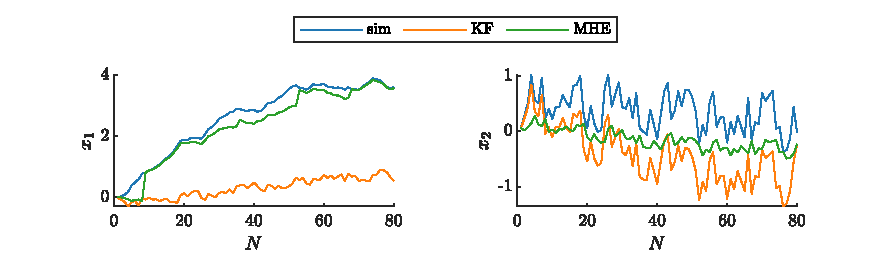
\includegraphics{figures/ex5_MHE.pdf}
\end{figure}

The cumulative squared errors for the two states using the two methods are as follows:
\begin{table}[!h]
    \centering
    \begin{tabular}{c|c|c}
        Method & $\tilde x_1$ & $\tilde x_2$ \\
        \hline 
        KF & 482.16 & 54.99 \\
        MHE & 7.98 & 27.72
    \end{tabular}
\end{table}

\clearpage
Comparing the performance of MHE and EKF, a model with non-linear perturbation ( given by (9) in the article) is used as an example and the results are as follows: 
\begin{figure}[!h]
    \centering
    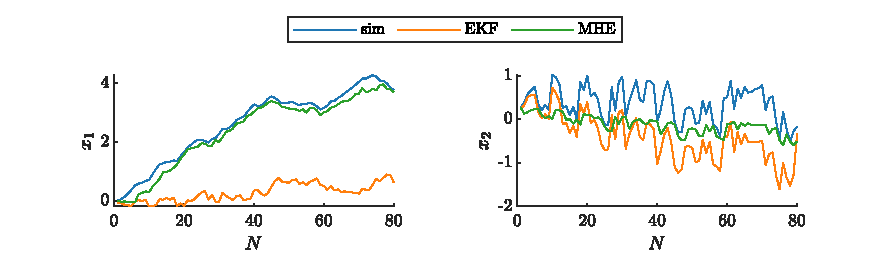
\includegraphics{figures/ex5_MHE_EKF.pdf}
\end{figure}

The cumulative squared errors for the two states using the two methods are as follows:
\begin{table}[!h]
    \centering
    \begin{tabular}{c|c|c}
        Method & $\tilde x_1$ & $\tilde x_2$ \\
        \hline 
        EKF & 187.08 & 61.39 \\
        MHE & 17.75 & 39.13
    \end{tabular}
\end{table}

